\chapter{Hardware Documentation}
\label{hardwareDocumentation}

\begin{figure}[H]
	\centering
	\includegraphics[width=16cm]{img/HWassembled.jpg}
	\label{HWassembled}
	\caption{Assembled SensorBoard prototype}
\end{figure}

\section{Overview}
SensorBoard is a prototype of autonomous hardware platform with microprocessor and various inertial, atmospheric and navigation sensors. The device can be used in many cases from logging data to movement control. The prototype works fully autonomously without connection to external power supply or other electronics, but allows wireless or wired connection to other electronic devices.

\subsection{Features}
\begin{itemize}
	\setlength\itemsep{0.2em}
	\item[--] No external power supply needed
	\item[--] Internal rechargeable battery
	\item[--] Charging from \ac{USB} or any \SI{5}{V} source
	\item[--] Allowed simultaneous connection to \ac{USB} and other power supply
	\item[--] Three different triaxial acceleromemers, dynamic gyroscopes and two different triaxial magnetometers
	\item[--] Barometer, light sensor, air humidity, temperature
	\item[--] A/D converters for connecting external sensors
	\item[--] TDOA location system with \SI{10}{cm} precission in \SI{300}{m} radius
	\item[--] External UART connector for GPS or radio communication
	\item[--] Hybrid WiFi and Bluetooth
	\item[--] Servo outputs and connector with other peripheries
	\item[--] User programmable dual core ESP32 processor
	\item[--] Various sleep modes to save battery power
	\item[--] More than 10 hours of operation from battery
	\item[--] Buttons and LEDs for interaction with user
	\item[--] Micro SD card up to \SI{32}{GB} for logging data (accessible from user program)
	\item[--] ARM Cortex-M0 co-processor for computing (sensor fusion, data analysis)
\end{itemize}

\subsection{Properties}

\begin{table}[H]
	\centering
	\begin{tcolorbox}[tab2,tabularx={|X|c|c|},title=SensorBoard properties]
		Parameter & Value & Unit \\
		\hline \hline
		Dimensions & 60 $\cdot$ 31 $\cdot$ 13 & mm \\
		Min Voltage & $-0.5$ & V \\
		Max Voltage & $5.5$ & V \\
		Max current & $2.1$ & A \\
		Max battery life & $12$ & hours \\
		WiFi antenna range & $10$ & m \\
		Bluetooth antenna range & $10$ & m \\
		TDOA location precission & $10$ & cm \\
		TDOA location range & $300$ & m \\
		Average charging time & $60$ & minutes \\
		Min temperature & $-10$ & \degree C \\
		Max temperature & $80$ & \degree C \\
	\end{tcolorbox}
	\caption{SensorBoard properties}
	\label{HWmaxRatings}
\end{table}

\subsection{Power Supply}
The SensorBoard can be powered from up to three independent power sources. The combination of more simultaneously connected supplies is allowed.

\begin{itemize}
	\item[--] \textbf{Internal battery:} The internal battery is a \ac{Li-poly} \SI{3.7}{V} (1S) accumulator. When no other supply is applied, the accumulator is used. There is an undervoltage protection of the battery. The SensorBoard can be switched off by hardware switch. The switch disconnects the battery, external supply can be still applied.
	\item[--] \textbf{\ac{USB} power supply:} When the \ac{USB} cable is connected, the \ac{Li-poly} accumulator is charging until the power consumption of the elctronics is lower than the maximal \ac{USB} supply. There is an overcharging protection of the battery.
	\item[--] \textbf{External \SI{5}{V} power:} The SensorBoard can be powered from an external \SI{5}{V} supply, for example from the servo connector. The \SI{5}{V} output on the board can be used as \SI{5}{V} power input as well.
\end{itemize}

\section{Getting Started}

\subsection{Assembling}
The device is assembled from three parts, two sandwich boards and one connector board. Optional devices like BMF055 board, GY953, HM-TRP or GPS can be connected to prepared ports. The parts are shown in figure \ref{HWassembling}.

\begin{figure}[H]
	\centering
	\includegraphics[scale=1]{img/assemblingHW.pdf}
	\label{HWassembling}
	\caption{Assembling the SensorBoard prototype}
\end{figure}

\subsection{Components Description}

\begin{figure}[H]
	\centering
	\includegraphics[scale=1]{img/componentsDescription.pdf}
	\label{HWcomponents}
	\caption{Components of the SensorBoard}
\end{figure}

\begin{table}[H]
	\centering
	\begin{tcolorbox}[tab2,tabularx={|c|X|c|},title=Description of components of the SensorBoard]
		Number & Description & Datasheet\\
		\hline \hline
		1 & DWM1000 location sensor & \cite{decawave:DWM1000} \\
		2 & BMF055 board connector (UART) & \cite{bosch:BMF055} \\
		3 & HM-TRP 433/868 MHz radio connector & \cite{HM-TRP} \\
		4 & Software buttons & \cite{TACTM} \\
		5 & GY-953 connector & \cite{GY953} \\
		6 & HM-TRP 433/868 MHz radio SMD pads & \cite{TACTM} \\
		7 & RPSMA antenna connector for HM-TRP radio & \cite{RPSMA} \\
		8 & External pins & Section \ref{pinNumbering} \\
		9 & Battery connector & Section \ref{pinNumbering} \\
		10 & Micro \ac{USB} connector with FTDI chip & \cite{ftdichip:FT232R} \\
		11 & ESP-WROOM-32 with WiFi/Bluetooth antenna & \cite{espressif:ESP-WROOM-32} \\
		12 & Micro SD card slot & \cite{MOLEX-SD1} \\
	\end{tcolorbox}
	\caption{Description of components of the SensorBoard}
	\label{table:componentsDescription}
\end{table}

\section{Pin Connections}

\subsection{Pin Numbering}
\label{pinNumbering}

\begin{figure}[H]
	\centering
	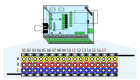
\includegraphics[scale=1]{img/externalPins.pdf}
	\caption{External pins numbering}
	\label{fig:externalPins}
\end{figure}

\begin{table}[H]
	\centering
	\begin{tcolorbox}[tab2,tabularx={|l||X|X|X|X|X|},title=External pins 01 -- 05]
		& 01 & 02 & 03 & 04 & 05 \\
		\hline \hline
		A & GND & +3V3 & SENSOR\_VP & SENSOR\_VN & IO33 \\ \hline
		B & \multicolumn{5}{c}{Pins B01 -- B17 internally connected, details in section \ref{jumpersExternalPins}} \\ \hline
		C & \multicolumn{5}{c}{GND} \\
	\end{tcolorbox}

	\vspace{0.5cm}
	
	\begin{tcolorbox}[tab2,tabularx={|l||X|X|X|X|X|X|X|X|X|X|X|X|},title=External pins 06 -- 17]
		& 06 & 07 & 08 & 09 & 10 & 11 & 12 & 13 & 14 & 15 & 16 & 17 \\
		\hline \hline
		A & IO25 & IO32 & IO26 & IO18 & IO19 & IO21 & IO16 & IO17 & IO23 & IO22 & IO27 & +5V \\ \hline
		B & \multicolumn{12}{c}{Pins B01 -- B17 internally connected, details in section \ref{jumpersExternalPins}} \\ \hline
		C & \multicolumn{12}{c}{GND} \\
	\end{tcolorbox}
	\caption{External pins mapping}
	\label{tab:externalPins}
\end{table}

\begin{table}[H]
	\centering
	\begin{tcolorbox}[tab2,tabularx={X|p{12cm}},title=Legend]
		Number          & Number of the pin corrsponding to figure \ref{fig:externalPins} and table \ref{tab:externalPins} \\
		Name            & Name of the pin corresponding to table \ref{tab:externalPins} \\
		Safety resistor & Yes if the \SI{220}{\ohm} safety resistor is present \\
		Pull-up         & Yes if the \SI{10}{k\ohm} pull-up resistor is present \\
		Part            & The pin is internally connected to which controller \\
		Pin             & The name of the controller's pin according to the datasheet \\
	\end{tcolorbox}

	\vspace{0.5cm}
	
	\begin{tcolorbox}[tab2,tabularx={|l|X|X|X|X|X|},title=External pins properties]
		Number & Name & Safety resistor & Pull-up & Part & Pin \\
		\hline \hline
		01 & GND & N/A & N/A & N/A & N/A \\
		02 & +3V3 & N/A & N/A & N/A & N/A \\
		03 & RADIO\_RX & Yes & No & ESP32 & SENSOR\_VP \\
		04 & RADIO\_TX & Yes & No & ESP32 & SENSOR\_VN \\
		05 & BTN1 & No & Yes & ESP32 & IO33 \\
		06 & BTN0 & No & Yes & ESP32 & IO25 \\
		07 & LED4 & Yes & No & ESP32 & IO32 \\
		08 & SCL0 & Yes & Yes & ESP32 & IO26 \\
		09 & SCK0 & Yes & No & ESP32 & IO18 \\
		10 & MISO0 & Yes & No & ESP32 & IO19 \\
		11 & MOSI0 & Yes & No & ESP32 & IO21 \\
		12 & MPU\_TX & Yes & No & ESP32 & IO16 \\
		13 & MPU\_RX & Yes & No & ESP32 & IO17 \\
		14 & CS\_DECA & Yes & No & ESP32 & IO23 \\
		15 & CS\_MPU2 & Yes & No & ESP32 & IO22 \\
		16 & SDA0 & Yes & No & ESP32 & IO27 \\
		17 & +5V & N/A & N/A & N/A & N/A \\
	\end{tcolorbox}
	\caption{External pins properties}
	\label{tab:externalPinsProperties}
\end{table}

\paragraph{Note:} Some external pins are not connected only to processor, but they are connected to other chips in parallel. The other chips are connected only via input only pins or with safety resistor. So, the possibility of damage by incorrect connection or by wrong software is minimized.

\subsection{Pin Description}
\begin{itemize}
	\setlength\itemsep{0.2em}
	\item[--] 01 -- \textbf{GND}: Ground
	\item[--] 02 -- \textbf{+3V3}: Power Supply \SI{+3.3}{V} from linear stabilizer
	\item[--] 03 -- \textbf{RADIO\_RX}: UART receive pin for external devices like radio communication or GPS
	\item[--] 04 -- \textbf{RADIO\_TX}: UART transmit pin for external devices like radio communication or GPS
	\item[--] 05 -- \textbf{BTN1}: Usage defined by user software, internally connected to button 1
	\item[--] 06 -- \textbf{BTN0}: Usage defined by user software, internally connected to button 0
	\item[--] 07 -- \textbf{LED4}: Usage defined by user software, internally connected to LED4
	\item[--] 08 -- \textbf{SCL0}: \itwoc clock pin for external devices, internally connected to sensors
	\item[--] 09 -- \textbf{SCK0}: SPI clock pin for external devices, internally connected to sensors
	\item[--] 10 -- \textbf{MISO0}: SPI data output pin for external devices, internally connected to sensors
	\item[--] 11 -- \textbf{MOSI0}: SPI data input pin for external devices, internally connected to sensors
	\item[--] 12 -- \textbf{MPU\_TX}: UART transmit pin for GY953 or external device
	\item[--] 13 -- \textbf{MPU\_RX}: UART receive pin for GY953 or external device
	\item[--] 14 -- \textbf{CS\_DECA}: Usage defined by user software, internally used as chip select pin for DWM1000 TDOA location sensor
	\item[--] 15 -- \textbf{CS\_MPU2}: Usage defined by user software, internally connected to GY953 port
	\item[--] 16 -- \textbf{SDA0}: \itwoc data pin for external devices, internally connected to sensors
	\item[--] 17 -- \textbf{+5V}: \SI{+5}{V} power supply from battery or \ac{USB} or external source, the battery voltage is converted to \SI{5}{V}
\end{itemize}

\paragraph{Note:} All pins except power supply pins can be redefined by software. Their new definition shouldn't be in collision with other connected parts. For details see figures \ref{sch1} and \ref{sch2}.

\subsection{Power Supply}
\label{jumpersExternalPins}
The pins B01 -- B17 are defined by jumpers. We usually need these pins connected to power supply. We can define the voltage by connecting arbitrary B pin to target power supply. The pins B01 -- B17 are internally connected, but they are not connected to anything else. We can define pins B01 -- 17 as:
\begin{itemize}
	\setlength\itemsep{0.2em}
	\item[--] \textbf{GND} by connecting A01 and B01 by jumper
	\item[--] \textbf{+3V3} by connecting A02 and B02 by jumper
	\item[--] \textbf{+5V} by connecting A17 and B17 by jumper
	\item[--] \textbf{anything} by connecting any B pin to our target
\end{itemize}

\begin{figure}[H]
	\centering
	\includegraphics[scale=1]{img/jumpers.pdf}
	\caption{Power supply definition by jumpers}
	\label{fig:jumpersSupply}
\end{figure}

\section{LED Meanings}

\begin{figure}[H]
	\centering
	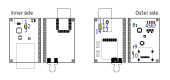
\includegraphics[scale=1]{img/LEDmeanings.pdf}
	\caption{SensorBoard LED meanings}
	\label{fig:LEDmeaning}
\end{figure}

\begin{enumerate}
	\setlength\itemsep{0.2em}
	\item \textbf{LED\_CBUS3}: (yellow) FTDI LED \cite{ftdichip:FT232R}, \ac{USB} power indication
	\item \textbf{LED\_CBUS2}: (yellow) FTDI LED \cite{ftdichip:FT232R}, \ac{USB} connection indication
	\item \textbf{LED\_CBUS4}: (yellow) FTDI LED \cite{ftdichip:FT232R}, \ac{USB} data transfer indication
	\item \textbf{LED\_5V}: (red) \SI{5}{V} power LED
	\item \textbf{LED\_3V3}: (red) \SI{3.3}{V} power LED
	\item \textbf{LED\_VCCIO}: (red) VCCIO power LED
	\item \textbf{LED\_USB}: (red) \ac{USB} power LED
	\item \textbf{LED6}: (green) Charging the battery indication
	\item \textbf{LED4}: (green) Software configurable LED
	\item \textbf{LED5}: (green) Software configurable LED
	\item \textbf{LED7}: (yellow) DWM1000 TXLED \cite{decawave:DWM1000}
	\item \textbf{LED3}: (yellow) DWM1000 RXLED \cite{decawave:DWM1000}
	\item \textbf{LED2}: (yellow) DWM1000 SFDLED \cite{decawave:DWM1000}
	\item \textbf{LED1}: (yellow) DWM1000 RXOKLED \cite{decawave:DWM1000}
\end{enumerate}

\section{Internal Connections}
The prototype of the SensorBoard contains several internal ports a lot of \ac{SMD} pads. The pads are designed mainly for testing. The connection of each pad can be found in the schematics and in the \ac{PCB} layout. The internal ports are dedicated for connection of internal devices that are not mounted on the board. The internal devices are battery, BMF055 \cite{bosch:BMF055} extension board and HM-TRP \cite{HM-TRP} radio.

The figure \ref{fig:internalConnection} and the table \ref{tab:internalConnection} describe all the internal ports. The yellow ports are designed for external connections and the grey ports are used for mechanical assembling. Only green ports are internal.

\begin{figure}[H]
	\centering
	\caption{Internal (green) and external (yellow) ports on the SensorBoard, the grey pins are used for mechanical assembling}
	\label{fig:internalConnection}
	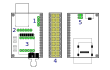
\includegraphics[scale=1]{img/pinSections.pdf}
\end{figure}

\begin{table}[H]
	\begin{tcolorbox}[tab2,tabularx={|c|c|X|},title=Internal and external ports on the SensorBoard]
		Number & Connection & Description \\ \hline
		1 & Internal & BMF055 board connector (UART) \\
		2 & Internal & HM-TRP 433/868 MHz radio connector \\
		3 & Internal & GY-953 connector \\
		4 & External & External pins \\
		5 & Internal & Battery connector \\
	\end{tcolorbox}
	\label{tab:internalConnection}
	\caption{Internal and external ports on the SensorBoard}
\end{table}

\subsection{Connector for BMF055 board (\ac{UART})}
The BMF055 connector is a \SI{3.3}{V} \ac{UART} connector. Its pinout is presented in figure \ref{fig:BMF055connectorBoard} and table \ref{tab:BMF055connectorBoard}.

\begin{figure}[H]
	\centering
	\label{fig:BMF055connectorBoard}
	\caption{Connector for BMF055 board (\ac{UART})}
	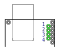
\includegraphics[scale=1]{img/BMFconnector.pdf}
\end{figure}

\begin{table}[H]
	\label{tab:BMF055connectorBoard}
	\caption{Connector for BMF055 board (\ac{UART})}
	\begin{tcolorbox}[tab2,tabularx={|c|c|X|},title=Connector for BMF055 board (\ac{UART})]
		Number & Name & Description \\ \hline
		1 & GND & Ground \\
		2 & +3V3 & \SI{3.3}{V} output \\
		3 & RX & Receive pin (\ac{UART}) \\
		4 & TX & Transmit pin (\ac{UART}) \\
	\end{tcolorbox}
\end{table}

\subsection{HM-TRP radio connector}
Pinout of the HM-TRP radio connector is presented in figure \ref{fig:HMTRPconnector} and table \ref{tab:HMTRPconnector}. The HM-TRP \cite{HM-TRP} radio is able to transmit or receive data at \SI{433}{MHz} or \SI{868}{MHz} frequency.

\begin{figure}[H]
	\centering
	\caption{HM-TRP radio connector}
	\label{fig:HMTRPconnector}
	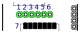
\includegraphics[scale=1]{img/HMTRPconnector.pdf}
\end{figure}

\begin{table}[H]
	\label{tab:HMTRPconnector}
	\caption{HM-TRP radio connector}
	\begin{tcolorbox}[tab2,tabularx={|c|c|X|},title=HM-TRP radio connector]
		Number & Name & Description \\ \hline
		1 & GND & Ground \\
		2 & CONFIG & Config pin, LOW for configuration mode, HIGH for communication \cite{HM-TRP} \\
		3 & +5V & \SI{5}{V} output \\
		4 & RX & Receive pin \\
		5 & TX & Transmit pin \\
		6 & ENABLE & Enable pin, LOW for normal mode, HIGH to sleep mode \\
		7 & SMD port & Port for \ac{SMD} version of the HM-TRP radio \cite{HM-TRP}, pinout in HM-TRP datasheet \\
	\end{tcolorbox}
\end{table}

\subsection{GY-953 connector}
Pinout of the GY-953 connector is presented in figure \ref{fig:GY953connector} and table \ref{tab:GY953connector}.

\begin{figure}[H]
	\centering
	\caption{GY-953 connector}
	\label{fig:GY953connector}
	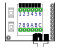
\includegraphics[scale=1]{img/GY953connector.pdf}
\end{figure}

\begin{table}[H]
	\label{tab:GY953connector}
	\caption{GY-953 connector}
	\begin{tcolorbox}[tab2,tabularx={|c|c|X|},title=GY-953 connector]
		Number & Name & Description \\ \hline
		1 & SWC & Serial Wire Clock (\ac{SWD} interface), not connected \\
		2 & SWD & Serial Wire Debug (\ac{SWD} interface), not connected \\
		3 & RX & Receive (\ac{UART}) \\
		4 & TX & Transmit (\ac{UART}) \\
		5 & GND & Ground \\
		6 & +5V & \SI{5}{V} output \\
		7 & B0 & Not connected \\
		8 & INT & Interrupt \\
		9 & MOSI & \ac{SPI} data out \\
		A & MISO & \ac{SPI} data in \\
		B & SCK & \ac{SPI} clock \\
		C & CS & \ac{SPI} chip select \\
	\end{tcolorbox}
\end{table}

\subsection{External pins}
The external port is discussed in section \ref{pinNumbering}.

\subsection{Battery connector}
Pinout of the battery connector is presented in figure \ref{fig:BATTconnector} and table \ref{tab:BATTconnector}.

\begin{figure}[H]
	\centering
	\caption{Battery connector}
	\label{fig:BATTconnector}
	
\includegraphics[scale=1]{img/BATTconnector.pdf}
\end{figure}

\begin{table}[H]
	\label{tab:BATTconnector}
	\caption{Battery connector}
	\begin{tcolorbox}[tab2,tabularx={|c|c|X|},title=Battery connector]
		Number & Name & Description \\ \hline
		1 & SWITCH\_A & ON/OFF switch (internally connected to BATT+) \\
		2 & SWITCH\_B & ON/OFF switch \\
		3 & BATT+ & Battery positive (internally connected to SWITCH\_A) \\
		4 & BATT- & Battery negative (Ground) \\
	\end{tcolorbox}
\end{table}

\section{BMF055 Extension Board}
\label{BMF055pinNumbering}
The BMF055 extension board contains the BMF055 chip \cite{bosch:BMF055} with its mandatory mainly \ac{RLC} accessories. The BMF055 chip wasn't placed directly onto the SensorBoard because it was very new on the market. I decided to use this chip, but to place it outside the main board. When any problem with the BMF055 chip occurs, I can simply disconnect this extension board from the main electronics.

\subsection{Pin Connection}
The pinout of the BMF055 extension board is shown in figure \ref{fig:BMF055pinout} and explained in table \ref{tab:BMF055pinout}.

\begin{figure}[H]
	\centering
	\caption{BMF055 extension board pinout}
	\label{fig:BMF055pinout}
	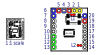
\includegraphics[scale=1]{img/BMF055pinout.pdf}
\end{figure}

\begin{table}[H]
	\label{tab:BMF055pinout}
	\caption{BMF055 extension board pinout}
	\begin{tcolorbox}[tab2,tabularx={|c|c|X|},title=BMF055 extension board pinout]
		Number & Name & Description \\ \hline
		1  & RX & \ac{UART} receive pin \\
		2  & TX & \ac{UART} transmit pin \\
		3  & VCC & \SI{3.3}{V} input/output supply \\
		4  & GND & Ground \\
		5  & VCC & \SI{3.3}{V} input/output supply \\
		6  & GND & Ground \\
		7  & GND & Ground \\
		8  & PB02 & Atmel SAM d20 GPIO (PB02) \cite{atmel:samd20} \\
		9  & PB01 & Atmel SAM d20 GPIO (PB01) \cite{atmel:samd20} \\
		10 & PB00 & Atmel SAM d20 GPIO (PB00) \cite{atmel:samd20} \\
		11 & SWD & \ac{SWD} interface, data pin \\
		12 & SWC & \ac{SWD} interface, clock pin \\
		13 & $\overline{RESET}$ & Reset when LOW \\
		14 & PA28 & Atmel SAM d20 GPIO (PA28) \cite{atmel:samd20} \\
		15 & PA23 & Atmel SAM d20 GPIO (PA23) \cite{atmel:samd20} \\
		16 & PA22 & Atmel SAM d20 GPIO (PA22) \cite{atmel:samd20} \\
		17 & PA21 & Atmel SAM d20 GPIO (PA21) \cite{atmel:samd20} \\
		18 & PA20 & Atmel SAM d20 GPIO (PA20) \cite{atmel:samd20} \\
		19 & VCC & \SI{3.3}{V} input/output supply \\
		20 & GND & Ground \\
	\end{tcolorbox}
\end{table}

\subsection{LED Meanings}
The BMF055 board has two \ac{LED}s, one power \ac{LED} and one software driven \ac{LED}. The positions of the \ac{LED}s are shown in figure \ref{fig:BMF055pinout} and marked as \texttt{L1} and \texttt{L2}. Their meaning is explained in table \ref{tab:BMF055leds}.

\begin{table}[H]
	\label{tab:BMF055leds}
	\caption{BMF055 extension board LED meaning}
	\begin{tcolorbox}[tab2,tabularx={|c|c|X|},title=BMF055 extension board LED meaning]
		Number & Name & Description \\ \hline
		L1 & Power LED & (red) The LED is ON if and only if the power is applied \\
		L2 & Software LED & (red) The LED is fully driven by firmware inside the BMF055 \\
	\end{tcolorbox}
\end{table}

\chapter{Schematics and PCB layout od the SensorBoard}
The schematics and the board layout was created in CadSoft EAGLE \cite{EAGLE}. The figures \ref{sch1} and \ref{sch2} shows the exported schematics split into two sheets. The exported \ac{PCB} layout drawing in scale 1:1 is in figure \ref{brd1} and in scale 2:1 with more details in figure \ref{brd2}.

\begin{figure}
	\centering
	\includegraphics[angle=90, width=\linewidth]{img/sch1.pdf}
	\label{sch1}
	\caption{Schematics of the SensorBoard sheet 1}
\end{figure}

\begin{figure}
	\centering
	\includegraphics[angle=90, width=\linewidth]{img/sch2.pdf}
	\label{sch2}
	\caption{Schematics of the SensorBoard sheet 2}
\end{figure}

\begin{figure}
	\centering
	\includegraphics[scale=1]{img/brd.pdf}
	\vspace{-0.5cm}
	\begin{center}
		Top and Bottom layer
	\end{center}
	\includegraphics[scale=1]{img/brdTop.pdf}
	\vspace{-0.5cm}
	\begin{center}
		Only Top layer
	\end{center}
	\includegraphics[scale=1]{img/brdBottom.pdf}
	\vspace{-0.5cm}
	\begin{center}
		Only Bottom layer
	\end{center}
	\label{brd1}
	\caption{SensorBoard layout in scale 1:1}
\end{figure}

\begin{figure}
	\centering
	\includegraphics[angle=90, scale=2]{img/brd.pdf}
	\label{brd2}
	\caption{SensorBoard layout in detail scale 2:1}
\end{figure}

\section{SensorBoard Drawings}
The SensorBoard drawings shows the correspondence between the manufactured prototype and its schematic drawings. The comparison is shown in figure \ref{fig:SensorBoardDrawings}.

\begin{figure}
	\centering
	\label{fig:SensorBoardDrawings}
	\caption{Drawings of the SensorBoard used in this paper}
	\includegraphics[width=\linewidth]{img/PCBphoto.jpg}
	\\Photo of the disassembled prototype\\
	\vspace{0.4cm}
	%\begin{minipage}[c]{.3\linewidth}
	%	\includegraphics[height=5cm]{img/renderBottom.png}
	%\end{minipage}
	%\quad
	%\begin{minipage}[c]{.3\linewidth}
	%	\includegraphics[height=5cm]{img/renderTop.png}
	%\end{minipage}
	%\quad
	%\begin{minipage}[c]{.15\linewidth}
	%	\includegraphics[height=2.5cm]{img/renderBMF.png}
	%\end{minipage}
	\includegraphics[width=\linewidth]{img/renders.png}
	\vspace{0.4cm}
	\\Renders of the \ac{PCB}\\
	\vspace{0.4cm}
	\includegraphics[scale=1]{img/SensorBoardDrawing.pdf}
	\\Schematical drawing
\end{figure}